\chapter{Integration strategy}\label{chap:strategy}



\section{Entry criteria}
% Specify the criteria that must be met before integration testing of specific elements may begin (e.g., functions must have been unit tested).
The first obvious condition which has to be satisfied before starting the integration test process is that the modules to be integrated are fully developed. Moreover, in order to provide a reliable background, most of the functions shall have already been unit tested. In detail, we require that at least \SI{75}{\percent} of each component to be integrated has been unit tested.\footnote{\color{red}ANDREA \`E RAGIONEVOLE?} 

It is also important that some mock data are created, in order to let the components work. Please, refer to \cref{chap:stubs} for further details.\footnote{\color{red}DEVO AGGIUNGERE ALTRO?}




\section{Elements to be integrated}
% Identify the components to be integrated, refer to your design document to identify such components in a way that is consistent with your design.
Integration testing deals with components. That is why in \cref{fig:component} we are showing the component diagram of myTaxiService system, already presented in section~2.3 of the \emph{Design document}.

\begin{figure*}%
	\centering% 
	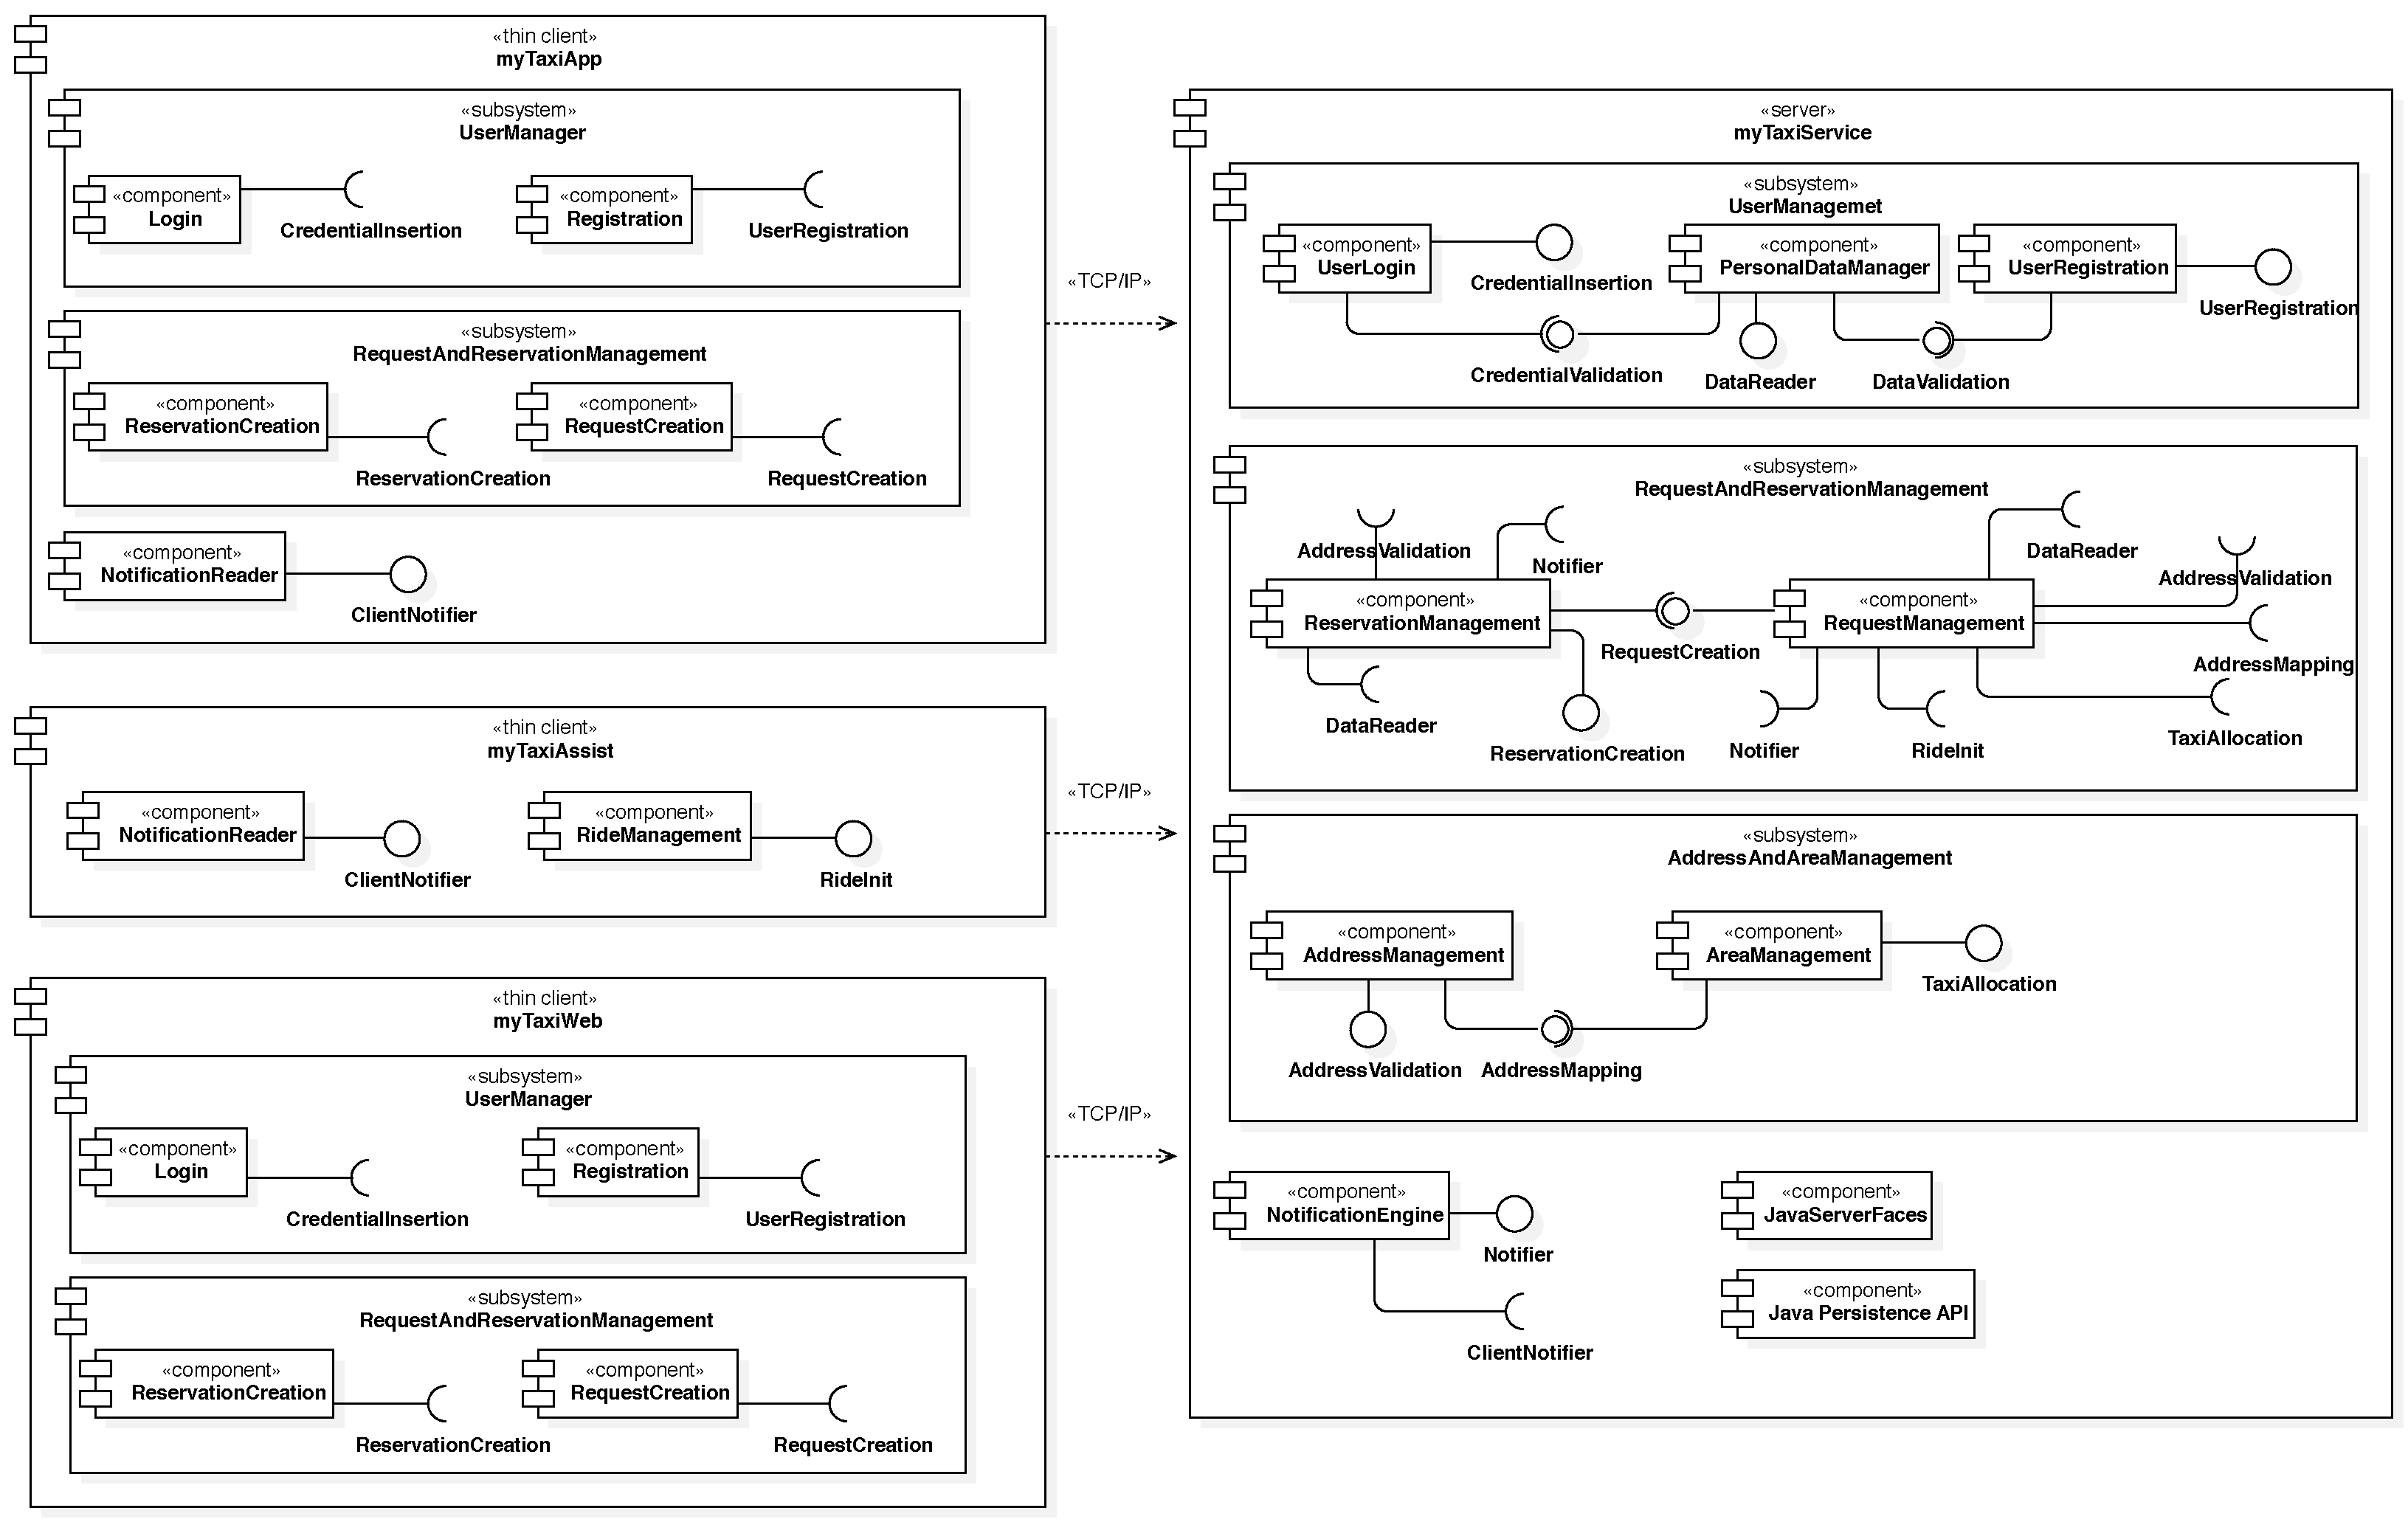
\includegraphics[width=\textwidth]{img/ComponentView__ComponentDiagram_1}%
	\caption{Component diagram.}%
	\label{fig:component}%
\end{figure*}

This testing plan covers most of the system, but some components are excluded. For instance, \texttt{User\-Login} and \texttt{User\-Registration} are left out, as they cope with security protocols and integration mechanisms, which would need a comprehensive document on their own. \texttt{Java\-Server\-Faces} and \texttt{Java Persistence API} are left out of this document, for similar reasons.



\section{Integration testing strategy}
% Describe the integration testing approach (top down, bottom up, functional groupings, etc.) and the rationale for the choosing that approach.
As of the strategy to adopt in order to complete the integration test, we select the \mbox{top-down} approach, which requires the \mbox{highest-level} modules (in terms of required functionalities and inclusions) be test and integrated first. This way a verified input is going to be provided to the following component or subsystem to be integrated.

This incremental approach, focused on the architecture of the system, may require some additional work, since stubs need to be created extensively, but nevertheless should be easy to understand and extend, and should arguably guarantee the quality of the software, \mbox{high-level} logic and data flow being tested early in the process.

At the end of the integration testing process, the system can be assumed as fully functional. As such, after undergoing a thorough system testing\footnote{Please notice that the planning of this process is outside the scope of this document.}, which shall include also careful performance assessments, can be released to users.
%TODO Is it, actually?





\section{Integration sequence}
%NOTE: The structure of this section may vary depending on the integration strategy you select in Section 2.3. Use the structure proposed below as a non mandatory guide.
%\subsection{Software Integration Sequence} For each subsystem: Identify the sequence in which the software components will be integrated within the subsystem. Relate this sequence to any product features/functions that are being built up.
%\subsection{Subsystem Integration Sequence} Identify the order in which subsystems will be integrated.
%If you have a single subsystem, 2.4.1 and 2.4.2 are to be merged in a single section. You can refer to Section 2.2 of the test plan example [1] as an example of what we expect.

In the following \cref{fig:intsequence} we present the actual sequence of integration to be followed, and reference details are provided in \cref{tab:intseq}.



\begin{figure*}%
	\centering%
	\includestandalone[width=\textwidth]{img/sequence/sequence_o}%  
	\caption{Sequence of integration.}%
	\label{fig:intsequence}%
\end{figure*}



\begin{table*}%
\centering%
\begin{tabularx}{.8\textwidth}{ >{\ttfamily\bfseries}c >{\ttfamily}X c }%
\toprule%
\normalfont\textsc{ID} & \normalfont\textsc{Integration test} & \normalfont\textsc{Reference} \\%
\toprule%
I1 & ReservationCreation $\to$ ReservationManagement & 3ref \\%
\midrule%
I2 & ReservationManagement $\to$ RequestCreation & 3ref \\%
\midrule%
I3 & RequestCreation{\normalfont{, }}AreaManagement $\to$ RequestManagement & 3ref \\%
\midrule%
I4 & RequestManagement $\to$ AddressManagement & 3ref \\%
\midrule%
I5 & AddressManagement $\to$ PersonalDataManagement & 3ref \\%
\midrule%
I6 & AddressManagement $\to$ NotificationEngine & 3ref \\%
\midrule%
I7 & PersonalDataManagement $\to$ RideManagement & 3ref \\%
\midrule%
I8 & Notification Engine $\to$ NotificationReader & 3ref \\%
\bottomrule%
\end{tabularx}%
\caption[][2em]{Integration sequence reference details.}%
\label{tab:intseq}%
\end{table*}














